\chapter{Fast Fourier Transformation mit Fensterung}\label{CFFTmF}
Im folgenden Kapitel wird eine FFT mit Fensterung beschrieben.
\section{Aufgabenstellung}\label{TFFTmF}
Um den Leckeffekt zu verringern kann man Fensterfunktionen verwenden. Hier soll die FFT nun mit einem gefensterten Signal verwendet werden.
\section{Durchführung}\label{DFFTmF}
Um die Fensterung zu realisieren haben wir in der 
main.c und in process\textunderscore data.c 
die entsprechenden Stellen durch Entfernen der Kommentarzeichen aktiviert.\\

\begin{adjustbox}{width=\textwidth, keepaspectratio} 
  \label{code:procdataKompFIR}
  \begin{lstlisting}[title=Codeausschnitt der modifizierten main.c]
	twidfftrad2_fr16(twiddle_table,FRAMELENGTH);
	gen_hamming_fr16(window,1,FRAMELENGTH);	/* Uncomment to generate Hamming window */
//	gen_bartlett_fr16(window,1,FRAMELENGTH);	/* Uncomment to generate Bartlett window */
	
\end{lstlisting}
\end{adjustbox}\\
\begin{adjustbox}{width=\textwidth, keepaspectratio} 
  \label{code:procdataKompFIR}
  \begin{lstlisting}[title=Codeausschnitt der modifizierten process\_data.c]
	winmul(pInFrame,window,FRAMELENGTH); /* uncomment to include window function */
\end{lstlisting}
\end{adjustbox}\\
Dies ruft die in der Vorbereitung erstellte Funktion winmul auf (vergleiche hierzu den Abschnitt Vorbereitung).
Zum Testen der Funktionalität legten wir ein Sinussignal mit 697Hz und einer Amplitude von 100mV an. 
\begin{figure}[H]
  \centering
    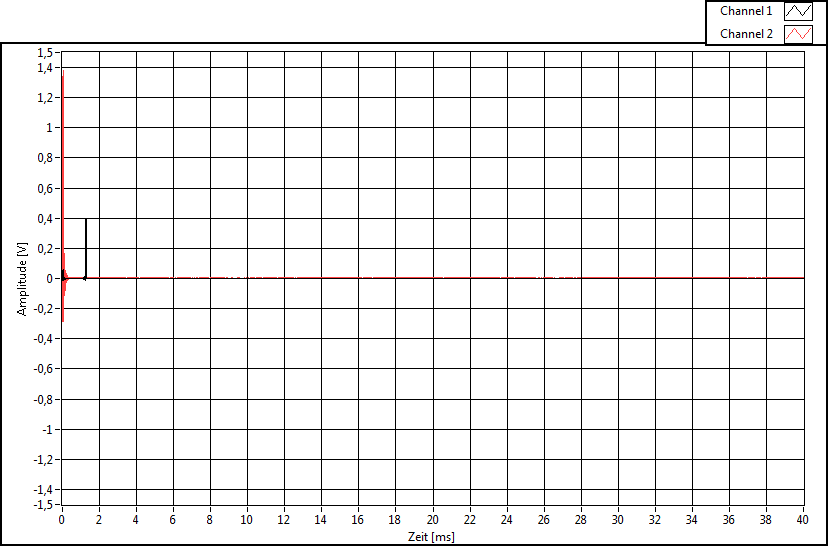
\includegraphics[width=\textwidth]{Hamming697Hz.png}
  \caption{Hammingfenster 697Hz 100mV}
  \label{fig:Hamming697Hz}
\end{figure}
Dies lieferte keinen sichtbaren Unterschied zu den vorherigen Versuchen, weshalb wir weiter hineinzoomten.
\begin{figure}[H]
  \centering
    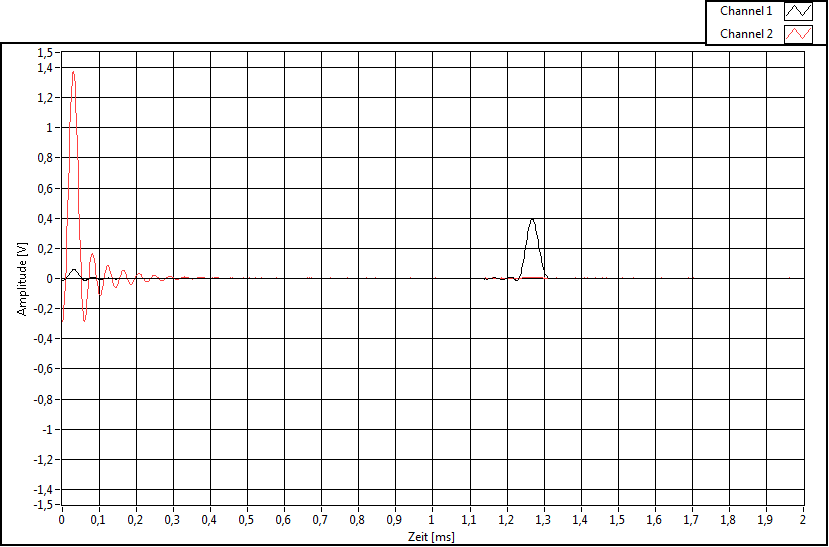
\includegraphics[width=\textwidth]{Hamming697Close.png}
  \caption{Hammingfenster 697Hz 100mV gezoomt}
  \label{fig:Hamming697Close}
\end{figure}
Da auch dies keine befriedigend sichtbare Verbesserung hervorbrachte haben wir in Matlab die Werte der FFT mit denen der gefensterten FFT grafisch übereinander gelegt.
\begin{figure}[H]
  \centering
    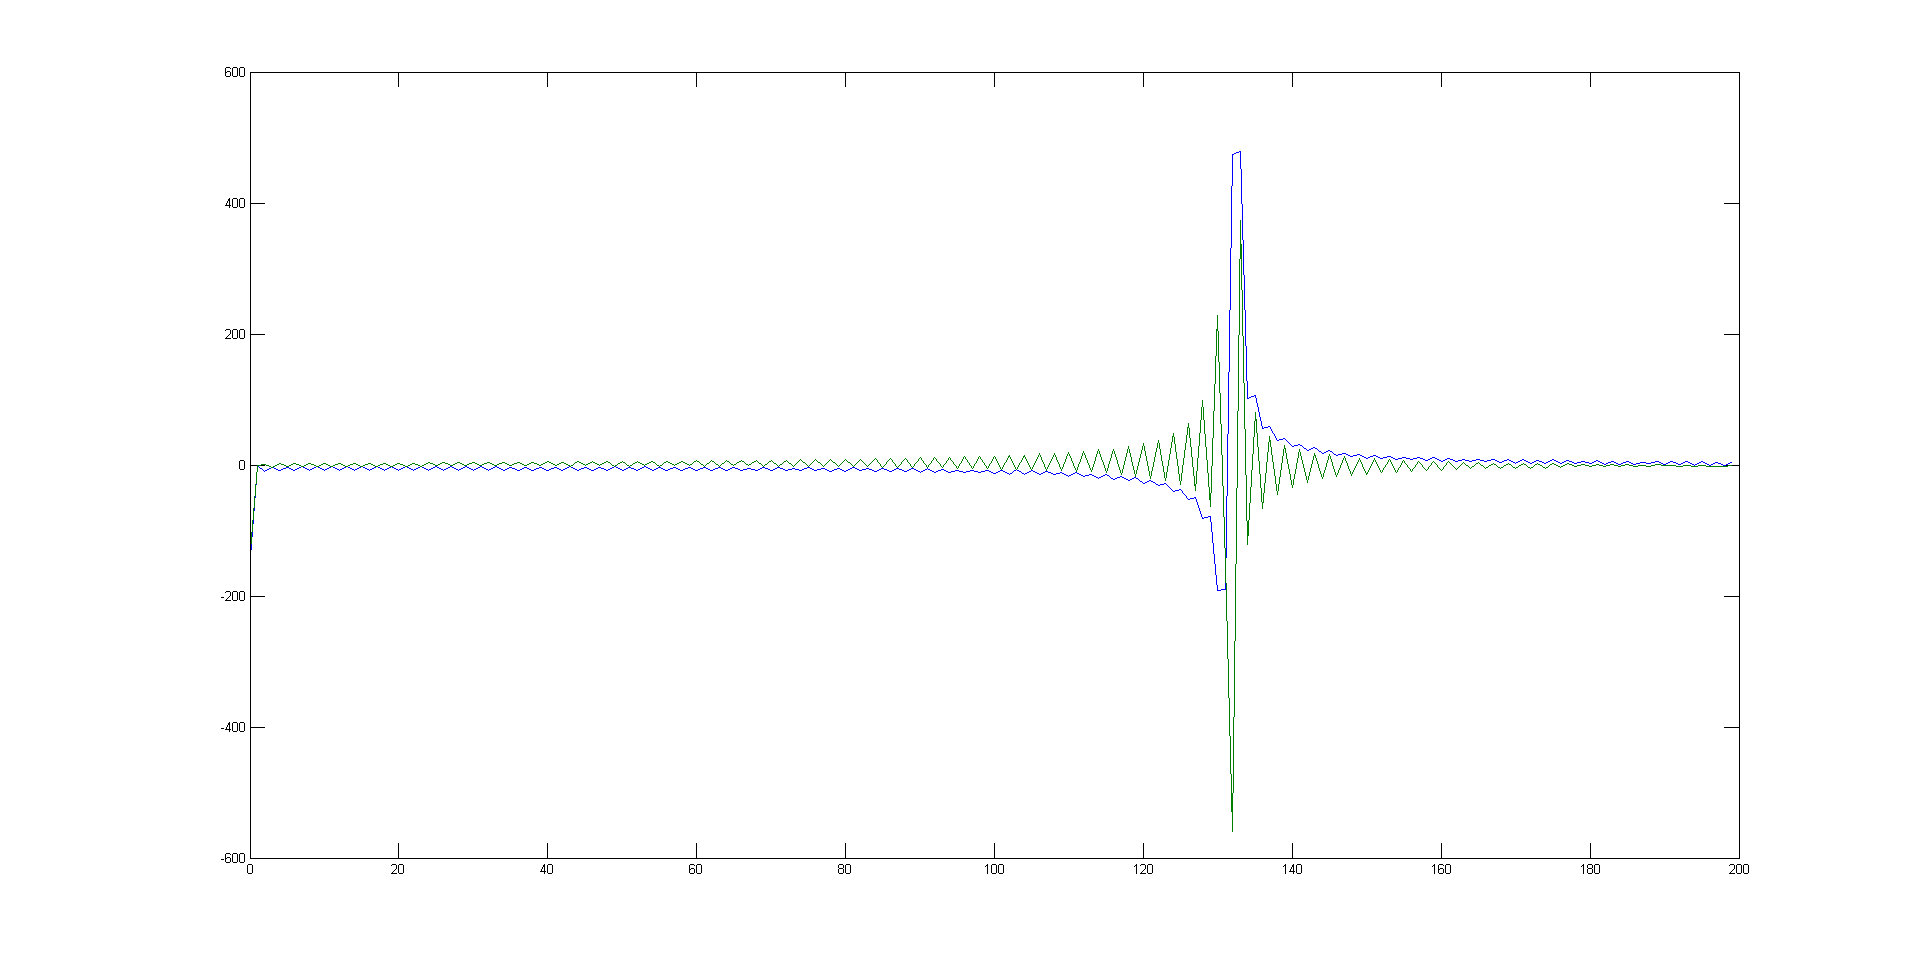
\includegraphics[width=\textwidth]{SpektrumImVergleich.png}
  \caption{Ausschnitt des Spektrums des Systems}
  \label{fig:SpektrumImVergleich}
\end{figure}
Es ist zu sehen dass die Werte die in den Speicherstellen des DSPs liegen sich sehr ähneln. Die negativen Werte erklären sich da in den Speicherstellen die komplexen Signalwerte liegen.

\section{Auswertung}\label{AFFTmF}
Dieses Ergebnis entspricht nicht unseren Erwartungen deckt sich aber mit den Ergebnissen des Bartlett-Fensters, die hier deshalb nicht extra aufgeführt werden. \\
Aus Zeitgründen haben wir dies in Absprache mit dem Übungsleites Herrn Professor Purat abgebrochen.\\
Wir hätten bei den gefensterten FFTs schmalere spektrallinien erwartet.